Bi-intuitionistic logic (BINT) is a conservative extension of
intuitionistic logic with perfect duality.  That is, BINT contains the
usual intuitionistic logical connectives such as true, conjunction,
and implication, but also their duals false, disjunction, and
coimplication. One leading question with respect to BINT is, what does
BINT look like across the three arcs -- logic, typed
$\lambda$-calculi, and category theory -- of the Curry-Howard-Lambek
correspondence?  A non-trivial (does not degenerate to a poset)
categorical model of BINT is currently an open problem.  This paper
directly contributes to the solution of this open problem by giving a
new categorical model based on adjunctions for cointuitionistic logic,
and then proposing a new categorical model for BINT.  In addition, we
give a new sequent calculus and term assignment for cointuitionistic
logic.

BINT can be seen as a mixing of two worlds: the first being
intuitionistic logic (IL), which is modeled categorically by a
cartesian closed category (CCC), and the second being the dual to
intuitionistic logic called cointuitionistic logic (coIL), which is
modeled by a cocartesian coclosed category (coCCC).  Crolard
\cite{Crolard:2001} showed that combining these two categories into
the same category results in it degenerating to a poset, that is,
there is at most one morphism between any two objects; we review this
result in
Section~\ref{subsec:cartesian_closed_and_cocartesian_coclosed_categories}.
However, this degeneration does not occur when both logics are linear.
We propose that IL and coIL need to be separated, and then mixed in a
control way using the modalities from linear logic.  This separation
can be ultimately achieved by an adjoint formalization of
bi-intuitionistic logic.  This formalization consists of three worlds
instead of two: the first is intuitionistic logic, the second is
linear bi-intuitionistic (Bi-ILL), and the third is cointuitionistic
logic.  They are then related via two adjunctions as depicted by the
following diagram:
\begin{center}
  \begin{tikzpicture}
    \node (img) {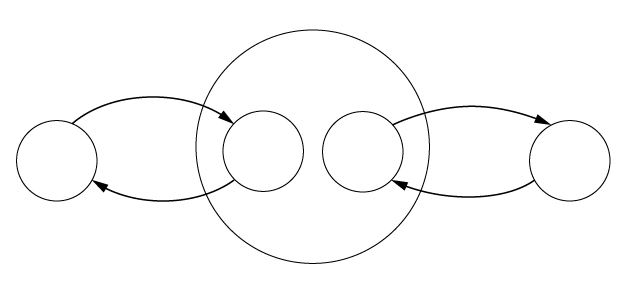
\includegraphics[scale=0.4]{introDiag}};
    \node (dv) at (-2.3, 0.0) {\huge $\dashv$};
    \node (IL) at (-3.58, -0.1) {IL};
    \node (vd) at (2.3, 0.0) {\huge $\vdash$};
    \node (coIL) at (3.65, -0.1) {coIL};

    \node (ILL) at (-0.67, 0.0) {ILL};
    \node (coILL) at (0.71, 0.0) {coILL};
    \node (BiILL) at (0, 1.0) {Bi-ILL};
  \end{tikzpicture}
    
\end{center}
The adjoint between IL and ILL is known as a LNL model of ILL, and is
due to Benton \cite{Benton:1994}.  However, the dual to LNL models
which would amount to the adjoint between coILL and coIL has yet to
appear in the literature.

The main contribution of this paper is the definition and study of the
dual to Benton's LNL models as models of cointuitionistic logic called
dual LNL models.  Bellin \cite{Bellin:2012} was the first to propose
the dual to Bierman's \cite{Bierman:1994} linear categories which he
names dual linear categories as a model of cointuitionistic linear
logic.  We conduct a similar analysis to that of Benton for dual LNL
models by showing that dual LNL models are dual linear categories
(Section~\ref{subsec:dual_lnl_model_implies_dual_category}), and that
from a dual linear category we may obtain a dual LNL model
(Section~\ref{subsec:dual_category_implies_dual_lnl_model}).
Following this we give the definition of bi-LNL models by combining
our dual LNL models with Benton's LNL models to obtain a categorical
model of bi-intuitionistic logic
(Section~\ref{subsec:a_mixed_bi-linear_non-linear_model}), but we
leave its analysis and corresponding logic to a future paper.
Following the categorical model we define and analyze a new sequent
calculus (Section~\ref{sec:sequent_calculus}), natural deduction
formalization (Section~\ref{sec:sequent-style_natural_deduction}), and
a term assignment (Section~\ref{sec:term_assignment}) for dual LNL
logic.

%%% Local Variables: 
%%% mode: latex
%%% TeX-master: main.tex
%%% End: 
